% Created by tikzDevice version 0.8.1 on 2015-05-25 07:51:41
% !TEX encoding = UTF-8 Unicode
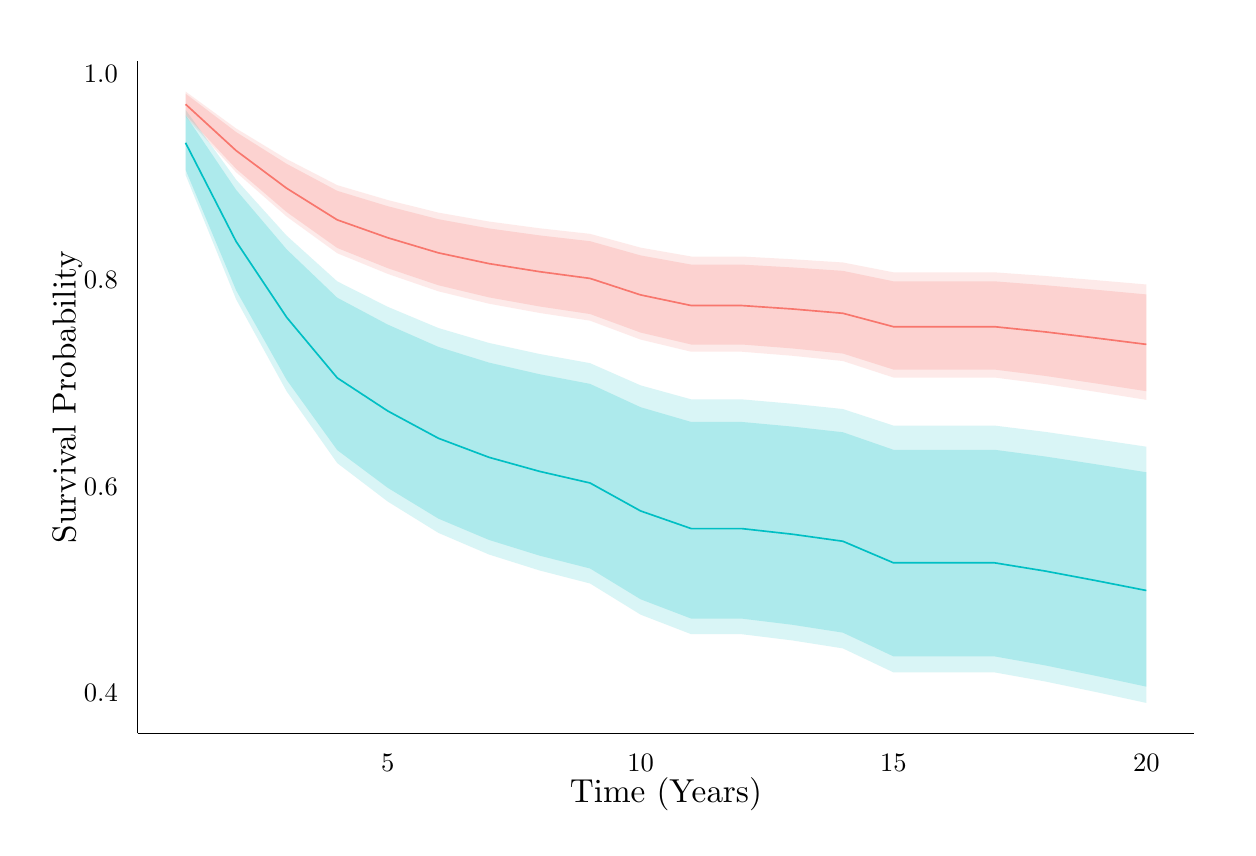
\begin{tikzpicture}[x=1pt,y=1pt]
\definecolor{fillColor}{RGB}{255,255,255}
\path[use as bounding box,fill=fillColor,fill opacity=0.00] (0,0) rectangle (433.62,289.08);
\begin{scope}
\path[clip] (  0.00,  0.00) rectangle (433.62,289.08);
\definecolor{drawColor}{RGB}{255,255,255}
\definecolor{fillColor}{RGB}{255,255,255}

\path[draw=drawColor,line width= 0.6pt,line join=round,line cap=round,fill=fillColor] (  0.00,  0.00) rectangle (433.62,289.08);
\end{scope}
\begin{scope}
\path[clip] ( 39.69, 34.03) rectangle (421.57,277.03);
\definecolor{fillColor}{RGB}{255,255,255}

\path[fill=fillColor] ( 39.69, 34.03) rectangle (421.58,277.03);
\definecolor{drawColor}{RGB}{248,118,109}

\path[draw=drawColor,line width= 0.6pt,line join=round] ( 57.05,261.41) --
	( 75.32,244.66) --
	( 93.59,231.04) --
	(111.86,219.63) --
	(130.13,213.16) --
	(148.41,207.71) --
	(166.68,203.82) --
	(184.95,200.91) --
	(203.22,198.47) --
	(221.49,192.51) --
	(239.77,188.67) --
	(258.04,188.67) --
	(276.31,187.43) --
	(294.58,185.87) --
	(312.86,181.02) --
	(331.13,181.02) --
	(349.40,181.02) --
	(367.67,179.15) --
	(385.94,176.95) --
	(404.22,174.64);
\definecolor{drawColor}{RGB}{0,191,196}

\path[draw=drawColor,line width= 0.6pt,line join=round] ( 57.05,247.46) --
	( 75.32,211.80) --
	( 93.59,184.40) --
	(111.86,162.53) --
	(130.13,150.56) --
	(148.41,140.71) --
	(166.68,133.83) --
	(184.95,128.75) --
	(203.22,124.55) --
	(221.49,114.44) --
	(239.77,108.07) --
	(258.04,108.07) --
	(276.31,106.04) --
	(294.58,103.49) --
	(312.86, 95.70) --
	(331.13, 95.70) --
	(349.40, 95.70) --
	(367.67, 92.73) --
	(385.94, 89.29) --
	(404.22, 85.70);
\definecolor{fillColor}{RGB}{248,118,109}

\path[fill=fillColor,fill opacity=0.15] ( 57.05,265.99) --
	( 75.32,252.66) --
	( 93.59,241.59) --
	(111.86,232.17) --
	(130.13,226.79) --
	(148.41,222.25) --
	(166.68,219.03) --
	(184.95,216.59) --
	(203.22,214.57) --
	(221.49,209.59) --
	(239.77,206.39) --
	(258.04,206.39) --
	(276.31,205.40) --
	(294.58,204.23) --
	(312.86,200.67) --
	(331.13,200.67) --
	(349.40,200.67) --
	(367.67,199.36) --
	(385.94,197.85) --
	(404.22,196.28) --
	(404.22,154.59) --
	(385.94,157.51) --
	(367.67,160.30) --
	(349.40,162.66) --
	(331.13,162.66) --
	(312.86,162.66) --
	(294.58,168.62) --
	(276.31,170.52) --
	(258.04,171.98) --
	(239.77,171.98) --
	(221.49,176.37) --
	(203.22,183.20) --
	(184.95,186.00) --
	(166.68,189.34) --
	(148.41,193.81) --
	(130.13,200.10) --
	(111.86,207.57) --
	( 93.59,220.82) --
	( 75.32,236.84) --
	( 57.05,256.89) --
	cycle;
\definecolor{fillColor}{RGB}{0,191,196}

\path[fill=fillColor,fill opacity=0.15] ( 57.05,259.40) --
	( 75.32,234.17) --
	( 93.59,213.91) --
	(111.86,197.41) --
	(130.13,188.20) --
	(148.41,180.55) --
	(166.68,175.16) --
	(184.95,171.17) --
	(203.22,167.85) --
	(221.49,159.82) --
	(239.77,154.77) --
	(258.04,154.77) --
	(276.31,153.18) --
	(294.58,151.27) --
	(312.86,145.29) --
	(331.13,145.29) --
	(349.40,145.29) --
	(367.67,143.02) --
	(385.94,140.39) --
	(404.22,137.67) --
	(404.22, 45.08) --
	(385.94, 49.03) --
	(367.67, 52.83) --
	(349.40, 56.11) --
	(331.13, 56.11) --
	(312.86, 56.11) --
	(294.58, 64.78) --
	(276.31, 67.66) --
	(258.04, 69.91) --
	(239.77, 69.91) --
	(221.49, 76.97) --
	(203.22, 88.23) --
	(184.95, 92.95) --
	(166.68, 98.71) --
	(148.41,106.52) --
	(130.13,117.83) --
	(111.86,131.74) --
	( 93.59,157.66) --
	( 75.32,190.92) --
	( 57.05,235.91) --
	cycle;
\definecolor{fillColor}{RGB}{248,118,109}

\path[fill=fillColor,fill opacity=0.20] ( 57.05,265.25) --
	( 75.32,251.36) --
	( 93.59,239.87) --
	(111.86,230.12) --
	(130.13,224.56) --
	(148.41,219.87) --
	(166.68,216.54) --
	(184.95,214.02) --
	(203.22,211.92) --
	(221.49,206.78) --
	(239.77,203.47) --
	(258.04,203.47) --
	(276.31,202.44) --
	(294.58,201.20) --
	(312.86,197.42) --
	(331.13,197.42) --
	(349.40,197.42) --
	(367.67,196.02) --
	(385.94,194.39) --
	(404.22,192.69) --
	(404.22,157.71) --
	(385.94,160.54) --
	(367.67,163.24) --
	(349.40,165.53) --
	(331.13,165.53) --
	(312.86,165.53) --
	(294.58,171.32) --
	(276.31,173.17) --
	(258.04,174.59) --
	(239.77,174.59) --
	(221.49,178.90) --
	(203.22,185.60) --
	(184.95,188.34) --
	(166.68,191.62) --
	(148.41,196.00) --
	(130.13,202.16) --
	(111.86,209.48) --
	( 93.59,222.44) --
	( 75.32,238.08) --
	( 57.05,257.61) --
	cycle;
\definecolor{fillColor}{RGB}{0,191,196}

\path[fill=fillColor,fill opacity=0.20] ( 57.05,257.45) --
	( 75.32,230.47) --
	( 93.59,208.97) --
	(111.86,191.50) --
	(130.13,181.78) --
	(148.41,173.73) --
	(166.68,168.06) --
	(184.95,163.86) --
	(203.22,160.36) --
	(221.49,151.93) --
	(239.77,146.61) --
	(258.04,146.61) --
	(276.31,144.93) --
	(294.58,142.89) --
	(312.86,136.55) --
	(331.13,136.55) --
	(349.40,136.55) --
	(367.67,134.13) --
	(385.94,131.33) --
	(404.22,128.43) --
	(404.22, 50.96) --
	(385.94, 54.87) --
	(367.67, 58.64) --
	(349.40, 61.89) --
	(331.13, 61.89) --
	(312.86, 61.89) --
	(294.58, 70.47) --
	(276.31, 73.31) --
	(258.04, 75.54) --
	(239.77, 75.54) --
	(221.49, 82.52) --
	(203.22, 93.65) --
	(184.95, 98.30) --
	(166.68,103.98) --
	(148.41,111.67) --
	(130.13,122.79) --
	(111.86,136.43) --
	( 93.59,161.79) --
	( 75.32,194.18) --
	( 57.05,237.74) --
	cycle;
\end{scope}
\begin{scope}
\path[clip] (  0.00,  0.00) rectangle (433.62,289.08);
\definecolor{drawColor}{RGB}{0,0,0}

\path[draw=drawColor,line width= 0.6pt,line join=round] ( 39.69, 34.03) --
	( 39.69,277.03);
\end{scope}
\begin{scope}
\path[clip] (  0.00,  0.00) rectangle (433.62,289.08);
\definecolor{drawColor}{RGB}{0,0,0}

\node[text=drawColor,anchor=base east,inner sep=0pt, outer sep=0pt, scale=  0.96] at ( 32.57, 45.54) {0.4};

\node[text=drawColor,anchor=base east,inner sep=0pt, outer sep=0pt, scale=  0.96] at ( 32.57,120.15) {0.6};

\node[text=drawColor,anchor=base east,inner sep=0pt, outer sep=0pt, scale=  0.96] at ( 32.57,194.77) {0.8};

\node[text=drawColor,anchor=base east,inner sep=0pt, outer sep=0pt, scale=  0.96] at ( 32.57,269.39) {1.0};
\end{scope}
\begin{scope}
\path[clip] (  0.00,  0.00) rectangle (433.62,289.08);
\definecolor{drawColor}{RGB}{0,0,0}

\path[draw=drawColor,line width= 0.6pt,line join=round] ( 39.69, 34.03) --
	(421.57, 34.03);
\end{scope}
\begin{scope}
\path[clip] (  0.00,  0.00) rectangle (433.62,289.08);
\definecolor{drawColor}{RGB}{0,0,0}

\node[text=drawColor,anchor=base,inner sep=0pt, outer sep=0pt, scale=  0.96] at (130.13, 20.31) {5};

\node[text=drawColor,anchor=base,inner sep=0pt, outer sep=0pt, scale=  0.96] at (221.49, 20.31) {10};

\node[text=drawColor,anchor=base,inner sep=0pt, outer sep=0pt, scale=  0.96] at (312.86, 20.31) {15};

\node[text=drawColor,anchor=base,inner sep=0pt, outer sep=0pt, scale=  0.96] at (404.22, 20.31) {20};
\end{scope}
\begin{scope}
\path[clip] (  0.00,  0.00) rectangle (433.62,289.08);
\definecolor{drawColor}{RGB}{0,0,0}

\node[text=drawColor,anchor=base,inner sep=0pt, outer sep=0pt, scale=  1.20] at (230.63,  9.03) {Time (Years)};
\end{scope}
\begin{scope}
\path[clip] (  0.00,  0.00) rectangle (433.62,289.08);
\definecolor{drawColor}{RGB}{0,0,0}

\node[text=drawColor,rotate= 90.00,anchor=base,inner sep=0pt, outer sep=0pt, scale=  1.20] at ( 17.30,155.53) {Survival Probability};
\end{scope}
\end{tikzpicture}
